\documentclass[../CSC_52081_EP.tex]{subfiles}

\begin{document}
    \section{Introduction}
    \label{sec:intro}

Reinforcement Learning (RL) has become a powerful paradigm for developing autonomous agents that learn optimal behaviors through interactions with their environments. In this study, we employ the CarRacing-v3 environment provided by Gymnasium \cite{gymnasium}, which presents a challenging control task in a racing scenario. The environment is characterized by a high-dimensional observation space and two distinct modes for the action space. Specifically, the observation space consists of a top-down \(96\times96\) RGB image capturing both the car and the racetrack, thus requiring the use of deep convolutional neural networks (CNNs) for effective feature extraction.

\begin{figure}[H]
    \centering
    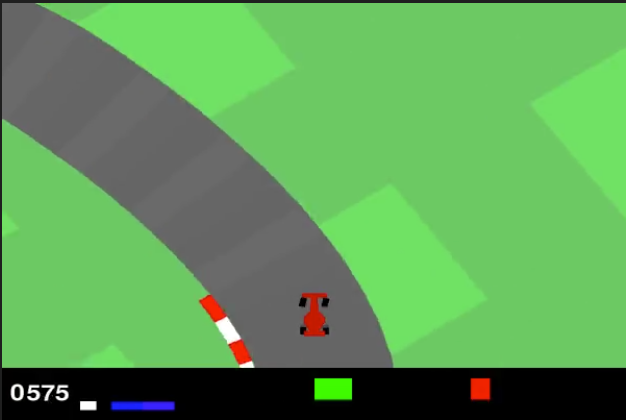
\includegraphics[scale = 0.3]{figures/car_racing_v3.png}
    \caption{A top-down 96x96 RGB image of the car and racetrack.}
    \label{fig:car_racing_v3}
\end{figure}

Regarding the action space, CarRacing-v3 supports both continuous and discrete control modalities. In the continuous mode, the agent outputs three real-valued commands: steering, where values range from \(-1\) (full left) to \(+1\) (full right); gas; and braking. Conversely, in the discrete mode, the action space is reduced to five actions: do nothing, steer left, steer right, gas, and brake. This duality in action representation allows for a comprehensive evaluation of various RL algorithms under different control settings.

The reward structure of the environment underscores the challenge by combining two components: a penalty of \(-0.1\) per frame and a reward of \(+\frac{1000}{N}\) for each new track tile visited, where \(N\) represents the total number of track tiles. For example, completing the race after visiting all \(N\) tiles in 732 frames, results in a reward of \(1000 - 0.1 \times 732 = 926.8\) points, as shown in \cite{gymnasium}. This scheme incentivize the agent to balance exploration (visiting tiles) with efficiency (minimizing frame usage), aligning its learning objectives with the task's overarching goal.

The primary objective of this project is to investigate and compare different RL policies across both discrete and continuous action modalities. For discrete action control, we implement methods such as Deep Q-Network (DQN) and SARSA. In contrast, for continuous action control, we explore approaches like the Cross-Entropy Method (CEM) and Self-Adaptive Evolution Strategy (SA-ES), and we also consider incorporating policy gradient techniques (e.g., Proximal Policy Optimization (PPO) and Soft Actor-Critic (SAC)). This comparative analysis is driven by our interest in understanding the strengths and limitations of each method in handling complex decision spaces.

The dual nature of the action space in CarRacing-v3 presents a significant challenge. When dealing with high-dimensional visual inputs, the necessity of effective feature extraction becomes paramount. To address this, our approach includes the development of a convolutional neural network architecture tailored to process the \(96\times96\) RGB images, reducing their dimensionality while preserving essential spatial features required for decision making. Additionally, transitioning between discrete and continuous representations of actions requires careful algorithmic design and parameter tuning to ensure stable learning and convergence.

While previous studies have applied various RL techniques in simulated environments, many have tended to focus on either discrete or continuous action spaces separately. In our work, we adopt a comparative approach by evaluating different agents within the same CarRacing-v3 environment. This allows us to assess the performance of each method under similar conditions, examining aspects such as learning stability, computational complexity, and overall policy effectiveness.

At this initial stage, this work primarily outlines the methodology and anticipated challenges, rather than presenting final empirical results. Our approach involves designing the CNN-based feature extractor, implementing the chosen RL algorithms, and setting up a robust framework for comparing their performances. While our preliminary findings are yet to be finalized, we expect that this study will offer valuable insights into the practical implications of employing RL in high-dimensional, real-time control tasks.

Specific limitations of the current work include the preliminary nature of our experiments and the need for further tuning and validation. Future work will focus on extensive empirical evaluations, exploring additional policy gradient methods, and refining the network architecture to better handle the complexities of the CarRacing-v3 environment.

The code for this project is available at \href{https://github.com/tr0fin0/ensta_CSC_52081_EP_project}{GitHub}, providing a reproducible framework for future investigations and extensions of this work.
\end{document}
